\documentclass[../main.tex]{subfiles}
\begin{document}
\section{Baseline Experiments}
\label{sec:baseline_experiments}

\subsection{Dataset}
The image dataset used in our work, which is obtained from the website of \href{https://kaggle.com/c/diabetic-retinopathy-detection}{Kaggle diabetic retinopathy competition} provided by EyePACS, contains 35126 high resolution fun- dus photographs taken under various imaging conditions. These fundus photographs have been labeled by a trained clinician with a scale of 0 to 4 based on the severity of DR. As a result, it is a typical five-class classification task where the model needs to correctly predict the severity of DR. 

Besides, it is noteworthy that these images are taken by different types of cameras under diverse conditions. Some of the images are inverted while some are incomplete due to the variant microscope imaging procedure. Also, noise in both images and labels is unavoidable in the raw data set, which puts forward a high demand to the robustness of our classification system. 

Last but not least, as shown in table \ref{table:label_partition}, the dataset is highly imbalanced. Consequently,  a "lazy" model which gives 0 as prediction all the time can achieve an accuracy of around 72\%. To show the capability of the model in classifying minor classes, we include \href{https://scikit-learn.org/stable/modules/generated/sklearn.metrics.balanced_accuracy_score.html}{ balanced accuracy} in our performance metrics.

\begin{table}[htbp]
\linespread{1.5}
\renewcommand\arraystretch{1.25}
\captionsetup{margin=5mm,justification=justified,font=small,labelfont=bf,textfont = it, margin={10mm,0mm}}
\centering
\begin{tabular}{|c|c|c|}
  \hline
    Label & Number of samples & Percentage\\
  \hline
    0 & 25810 & 73.5\% \\
    \hline
    1 & 2443 & 6.9\%\\
    \hline
    2 & 5292 & 15.1\%\\
    \hline
    3 & 873 & 2.5\%\\
    \hline
    4 & 708 & 2.0\% \\
    \hline
\end{tabular}
\caption{Distribution of original dataset}
\label{table:label_partition}   
\end{table}

\subsection{Image Preprocessing and Data Augmentation}
\textbf{Image Augmentation}. As mentioned above, the raw fundus images in the dataset have large variations in terms of brightness, contrast and the colour of eyeballs. Such irregularities constitute noise to the model and thus prevent it from effectively learning meaningful features. In order to standardise these images and reduce artifacts produced by irrelevant factors, we refer to the preprocessing scheme proposed by competition winner \href{https://storage.googleapis.com/kaggle-forum-message-attachments/88655/2795/competitionreport.pdf}{Graham}. More precisely, we subtract each pixel value of images by the weighted means of its surrounding pixel values, and add it by 50\% grayscale. This operation is similar to the ‘high pass’ processing in the PhotoShop software, which makes the blood vessels as well as the lesion areas in fundus images more explicit. Then, the fundus area in images will be clipped to 95\% of the original size by covering a mask with a transparent circle on the center in order to remove the boundary effects arising from the last operation. Afterwards, pixel values of images are normalised to [-1 , 1]. Effects of the preprocessing procedure are demonstrated in figure \ref{fig:preprocessed}. 

\begin{figure}[htbp]
\captionsetup{margin=5mm,justification=justified,font=small,labelfont=bf,textfont = it, margin={10mm,0mm}}
\centering
\begin{minipage}{7cm}
\centering
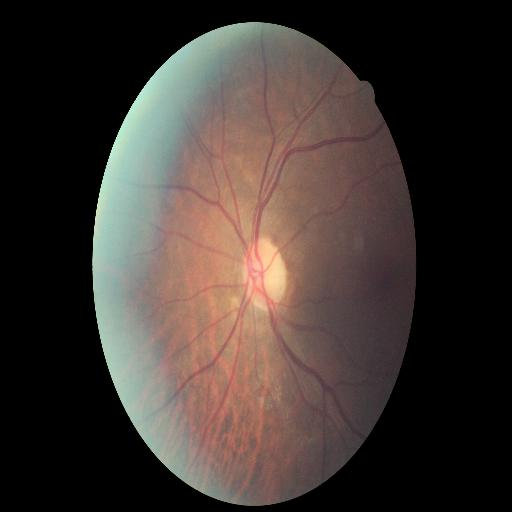
\includegraphics[width=0.8\textwidth]{original.jpeg}
\subcaption{original image}
\end{minipage}
\begin{minipage}{7cm}
\centering
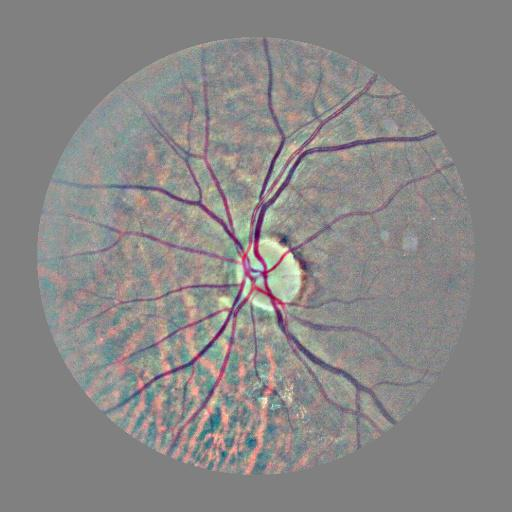
\includegraphics[width=0.8\textwidth]{preprocessed.jpeg}
\subcaption{processed image}
\end{minipage}
\caption{Comparison between a typical original image and a typical preprocessed image. it can be found that fundus region is standardized to be a circular area, containing the optic disk, macula and main vessels. Furthermore, the background color of retina is faded, while the venules, hard exudates and hemorrhages are emphasized.}
\label{fig:preprocessed}
\end{figure}

\textbf{Image Resize}. The original images in the dataset are of different sizes around 3k$\times$2k. Loading a dataset with images of such resolution exceeds the capacity of the gpu memory and the the inconsistency of the resolution makes it impossible to train a model using the raw images. Consequently, we resize them to 256$\times$256. Initially, the resizing is done "on the fly", which means that the images are modified upon being read for training. This brought much repeated and unnecessary work and slowed down the training. For the sake of improvement, we resize the images and save them as a new dataset and directly train the model on it. In this way the training is sped up by around 73 times.

\textbf{Data Augmentation}. In order to enhance diversity of the dataset and therefore alleviate the problem of overfitting, we further apply various transformations to the images fed to the model during training, which includes:
\begin{itemize}
  \item Randomly flip the images of left eye and right eye horizontally. Since human eyes are structurally mirror-symmetric, the fundus images can be flipped horizontally without affecting the label they correspond to.
  \item Randomly perform geometric transformation on images, including randomly scaling to 90\%-110\% of their size, translating by $\pm$0.05\% of the total width, rotating from -30 to 10 degrees and shearing from -10 to 10 degrees.
  \item Randomly change the brightness to 85\%-115\%, decreasing or improving the contrast in the range of 85\%-115\%.
\end{itemize}
All the steps of augmentation listed above are performed with a probability of 50\%.

\subsection{Model Architecture}
\textbf{Model Architecture}. For this typical image classification task, we employ two popular network structure families: resnet\cite{he_deep_2015}, efficientnet\cite{tan_efficientnet_2019} and InceptionV3\cite{szegedy_rethinking_2015}. For the resnet family, resnet18 and resnet50 are used while for the efficientnet family we use efficientnet b0 - b3. Table\ref{tab:num_parameters} shows the number of parameters of different networks. We also make use of transfer learning which consists in replacing the classification layer with a 5-unit one and in loading pretrained weights of the mentioned networks on Imagenet before the start of training. 

\begin{table}[htbp]
\linespread{1.5}
\renewcommand\arraystretch{1.25}
\captionsetup{margin=5mm,justification=justified,font=small,labelfont=bf,textfont = it, margin={10mm,0mm}}
\centering
\begin{tabular}{|c|c|}
  \hline
    Model & Number of Params \\
  \hline
    resnet18 & 11179077($\sim$11M)\\
    \hline
    resnet50 & 23518277($\sim$23M)\\
    \hline
    efficientnet b0 & 4013953($\sim$4M)\\
    \hline
    efficientnet b1 & 6519589($\sim$6M)\\
    \hline
    efficientnet b2 & 7708039($\sim$7M)\\
    \hline
    efficientnet b3 &10703917($\sim$10M) \\
    \hline
    InceptionV3 & 24357354($\sim$24M) \\
    \hline
\end{tabular}
\caption{Number of parameters of different models}
\label{tab:num_parameters}   
\end{table}
    

\subsection{Evaluation Methods and Results}
To assess the performance of models tested, the original dataset is split into training set and validation set with a ratio of 7:3 and the resulting datasets are used throughout the whole series of experiments. Since the split is random, the resulting datasets approximately preserve the distribution of the original dataset(table\ref{tab:training_dist}). 

To compare the performance of the models obtained with Kaggle competitors, Quadratic weighted kappa score is adopted as one of the evaluation metrics. It is able to describe the agreement between predicted labels and true labels more effectively, since it cost-sensitively penalizes the wrong predictions in terms of the degree of classification error. It ranges from 0 to 1 and is the higher the better. 

Training epochs are all set to be 20. Training is performed on 3 Tesla K40c gpus and the batch size is adjusted such that it is the greatest that does not exceed the memory capacity of the gpus. As for implementations, the balanced accuracy and cohen kappa score are calculated using corresponding sklearn functionalities and the deep learning library employed is Pytorch. 

We test the model on the validation set after each epoch. The results shown in table\ref{tab:test performance} are the ones at the best epoch(early stopping). Several observations can be made:
\begin{itemize}
  \item The models have better performance on images with higher resolution(512$\times$512 in our case).
  \item The efficientnet family has a better performance than the resnet family with much less parameters.
  \item efficientnets with image size of 512$\times$512 achieves a cohen kappa score comparable to the top teams in the kaggle competition leaderboard (for reference, the score of $10^{th}$ team is 0.814.)
  \item \href{https://github.com/lukemelas/EfficientNet-PyTorch}{The implementation of efficientnet in pytorch} is not memory efficient thus the allowed batch size is much smaller than it should be, which results in a longer training time. 
\end{itemize}
Considering training time and performance, we select efficient b0 as the baseline model and use image size of 512$\times$512 for the following experiments. 

\begin{table}[!htb]
    \linespread{1.5}
\renewcommand\arraystretch{1.25}
\captionsetup{margin=5mm,justification=justified,font=small,labelfont=bf,textfont = it, margin={10mm,0mm}}
    \begin{subtable}{.5\linewidth}
      \centering
\begin{tabular}{|c|c|c|}
  \hline
    Label & Number of samples & Percentage\\
  \hline
    0 & 18134 & 73.8\% \\
    \hline
    1 & 1710 & 6.9\%\\
    \hline
    2 & 3659 & 14.8\%\\
    \hline
    3 & 603 & 2.5\%\\
    \hline
    4 & 480 & 2.0\% \\
    \hline
\end{tabular}
    \caption{}
    \end{subtable}%
    \begin{subtable}{.5\linewidth}
      \centering
\begin{tabular}{|c|c|c|}
  \hline
    Label & Number of samples & Percentage\\
  \hline
    0 & 7673 & 72.9\% \\
    \hline
    1 & 733 & 6.9\%\\
    \hline
    2 & 1632 & 15.5\%\\
    \hline
    3 & 270 & 2.5\%\\
    \hline
    4 & 228 & 2.2\% \\
    \hline
\end{tabular}
    \caption{}
    \end{subtable} 
        \caption{Distribution of training dataset(a) and validation dataset(b)}
        \label{tab:training_dist}
\end{table}

\begin{table}[htbp]
\linespread{1.5} 
\renewcommand\arraystretch{1.25}
\captionsetup{margin=5mm,justification=justified,font=small,labelfont=bf,textfont = it, margin={10mm,0mm}}
\centering
\begin{tabular}{|c|c|c|c|c|c|c|}
    \hline
     \textbf   & Image Size  & Batch Size & Accuracy & Balanced Accuracy & Cohen Kappa Score & Training Time(20 epochs)\\
     \hline
     resnet18   &   256$\times$256 & 128 & 0.812 & 0.476 & 0.701 & 2h40min         \\
     \hline
     resnet18  &   512$\times$512  & 64 & 0.836 & 0.521 & 0.760 & 8h26min       \\
     \hline
     resnet50  &  256$\times$256 & 64 & 0.819 & 0.519 & 0.725   & 5h59min       \\
     \hline
     resnet50  &  512$\times$512 & 64 & 0.826 & 0.467 & 0.725    & 19h25min      \\
     \hline
     efficientnetb0 & 256$\times$256 & 192 & 0.815 & 0.440 & 0.696 & 2h29min  \\
     \hline
     efficientnetb0 & 512$\times$512 & 16 & \textbf{0.852} & 0.586 & 0.805 & 14h59min\\
     \hline
     efficientnetb1 & 256$\times$256 & 192 & 0.817 & 0.455 & 0.706 & 2h29min  \\ 
     \hline
     efficientnetb1 & 512$\times$512 & 16 & 0.850 & 0.587 & 0.805 & 19h15min  \\
     \hline
     efficientnetb2 & 256$\times$256 & 96 & 0.823 & 0.549 & 0.739 & 2h20min \\
     \hline
     efficientnetb2 & 512$\times$512 & 16 & \textbf{0.852} & \textbf{0.610} & \textbf{0.811} & 19h49min \\
     \hline
     efficientnetb3 & 256$\times$256 & 96 & 0.828 & 0.539 & 0.746 & 5h50min \\
     \hline
     efficientnetb3 & 512$\times$512 & 24 & 0.851 & 0.585 & 0.803 & 10h1min \\
     \hline
     InceptionV3 & 299$\times$299 & 64 & 0.816 & 0.497 & 0.706 & 7h12min \\
     \hline
\end{tabular}
\caption{Performance of different models}
\label{tab:test performance}   
\end{table}

%------------------------------------------Dataset Balancing--------------------------------------------------------------------
\section{Dataset Balancing}
The model obtained in section\ref{sec:baseline_experiments} is trained on an imbalanced dataset. Therefore, the distribution of the prediction is also imbalanced and significantly leans to the major class (i.e. class with label 0). This effect can be seen in figure\ref{fig:confusion_imbalanced}(a) which is the confusion matrix of efficient b0 tested on the validation set. In practice, this implies that patients with with DR would be wrongly diagnosed as Non-DR, which would cause a delay of treatment and aggravate the illness. From the point of view of robustness, the decision boundary of the dominant class  is considerably large and accordingly the one of the minor class is tiny and brittle: a small perturbation to the images with minor label leads to a change in prediction, which makes the model non robust. 

In order to alleviate this model learning bias, we extensively experiment with two families of dataset-balancing methods: Modify loss to give more emphasis on the minority classes and rebalance the class prior distributions in a pre-processing procedure. In detail, 
\begin{itemize}
\item{Loss Modification}
\begin{itemize}
\item Focal Loss\cite{lin_focal_2018}
\item Class balanced loss\cite{cui_class-balanced_2019}
\item Inverse Frequency Loss (The loss of images is reweighed by the inverse of the frequency of the class they represent.)
\end{itemize}
\item{Dataset Balancing}
\begin{itemize}
\item Oversampling(Add repeated minor class samples until all classes have the same number of samples. The resulting dataset in our case counts 103240(25810*5) samples in total.)
\end{itemize}
\end{itemize}

\subsection{Results}
The results of various methods are listed in table\ref{tab:balancing}. The setting is the same as section\ref{sec:baseline_experiments} and the model used is efficientnet b0. Some observations are made:
\begin{itemize}
  \item In spite of data augmentation, training on an oversampled dataset exhibits model overfitting probably owing to repeatedly visiting duplicated samples. Overfitting causes a sharp drop in model performance. Although the problem of overfitting can be mitigated through dropout, judging from the confusion matrix (figure\ref{fig:confusion_imbalanced}(b)), the resulting model has a distribution of decision similar to the one trained on imbalanced dataset but with a lower accuracy in predicting the major class. In addition, due to drastic increase of number of samples (from 20k to 100k), the training time climbs considerably. 
  \item If one starts the training from a pre-trained weight obtained from the above baseline experiments and applies oversampling, the model still overfits but at the first few epochs its decision distribution becomes more balanced(figure\ref{fig:confusion_imbalanced}(c)) at the expense of prediction accuracy of the major class and the overall accuracy stays at an acceptable level. The shown confusion matrix is that of the model obtained after 1 epoch of training.
  \item On the contrary, training with a reweighed loss function helps to balance decision distribution without overfitting problem and the training is notably faster than oversampling. Overall, focal loss with $\gamma$=2 and class balanced loss with $\beta$=0.99 would be good choices among all tested loss functions since they yield the highest balanced accuracy with merely a minor loss in normal accuracy. According to the confusion matrix they result in (figure\ref{fig:confusion_imbalanced}(d, e)), they successfully force the model to attach more importance to minor classes, which results in a better accuracy in predicting certain minor classes. However, they have little influence on balancing the decision distribution and it can still be found that the model tends to give 0 as prediction.
\end{itemize}

\begin{table}[htbp]
\linespread{1.5} 
\renewcommand\arraystretch{1.25}
\captionsetup{margin=5mm,justification=justified,font=small,labelfont=bf,textfont = it, margin={10mm,0mm}}
\centering
\begin{tabular}{|c|c|c|c|c|c|}
    \hline
     \textbf   & Batch Size & Accuracy & Balanced Accuracy & Cohen Kappa Score & Training Time (20 epochs)\\
     \hline
     crossentropy(baseline)   & 16 & 0.852 & 0.586 & 0.805  &   14h59min    \\
     \hline
     focal loss@$\gamma$=1  & 48 & 0.847 & 0.587 & 0.800    & 6h02min   \\
     \hline
     focal loss@$\gamma$=2   & 48 & 0.848 & \textbf{0.629} & 0.814   & 6h08min     \\
     \hline
     focal loss@$\gamma$=3   & 48 & 0.843 & 0.602 & \textbf{0.815}  & 6h12min    \\
     \hline
     focal loss@$\gamma$=4  & 48 & 0.842 & 0.593 & 0.803 & 5h50min  \\
     \hline
     class balanced loss@$\beta$=0.9  & 48 & 0.848 & 0.597 & 0.809 & 6h05min\\
     \hline
     class balanced loss@$\beta$=0.99  & 48 & \textbf{0.852} & 0.621 & 0.802  & 6h09min\\ 
     \hline
     class balanced loss@$\beta$=0.999  & 48 & 0.848 & 0.605 & 0.807  & 6h20min\\
     \hline
     inverse frequency loss & 16 & 0.798 & 0.596 & 0.764 & 14h30min\\
     \hline
     oversampling+dropout=0 & 16 & 0.704 & 0.399 & 0.612 & 46h39min\\
     \hline
     oversampling+dropout=0.75 & 48 &0.826&0.555&0.775 & 21h37min\\
     \hline
     oversampling+dropout=0.9 & 48 &0.780&0.578&0.780 & 20h05min\\
     \hline
     oversampling+restart & 48 & 0.760 &0.630 &0.765 & 5h4min (5 epochs) \\
     \hline
\end{tabular}
\caption{Performance of efficient b0 under different balancing methods}
\label{tab:balancing}
\end{table}

\begin{figure}[htbp]
\captionsetup{margin=5mm,justification=justified,font=small,labelfont=bf,textfont = it, margin={10mm,0mm}}
\centering
\begin{minipage}{5cm}
\centering
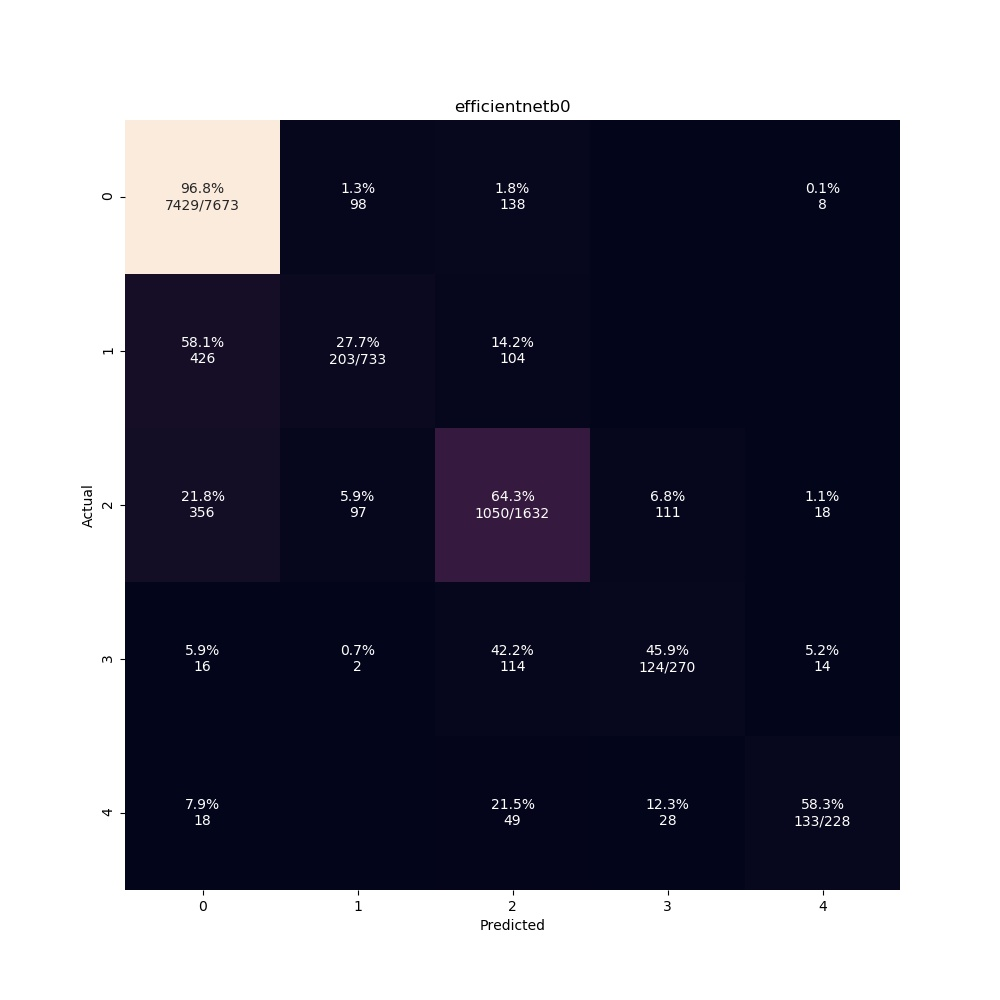
\includegraphics[width=1\linewidth]{efficientnetb0.jpeg}
\subcaption{}
\end{minipage}
\begin{minipage}{5cm}
\centering
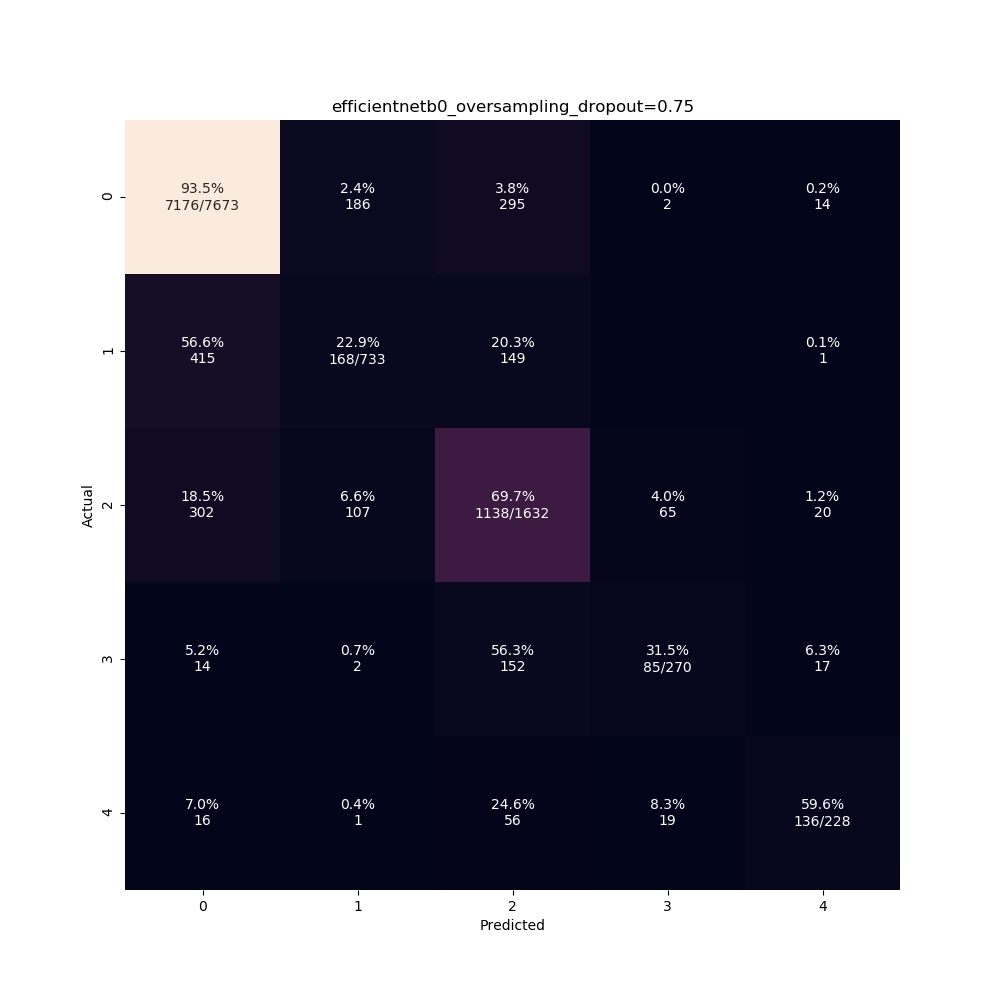
\includegraphics[width=1\linewidth]{efficientnetb0_oversampling_dropout.jpeg}
\subcaption{}
\end{minipage}
\begin{minipage}{5cm}
\centering
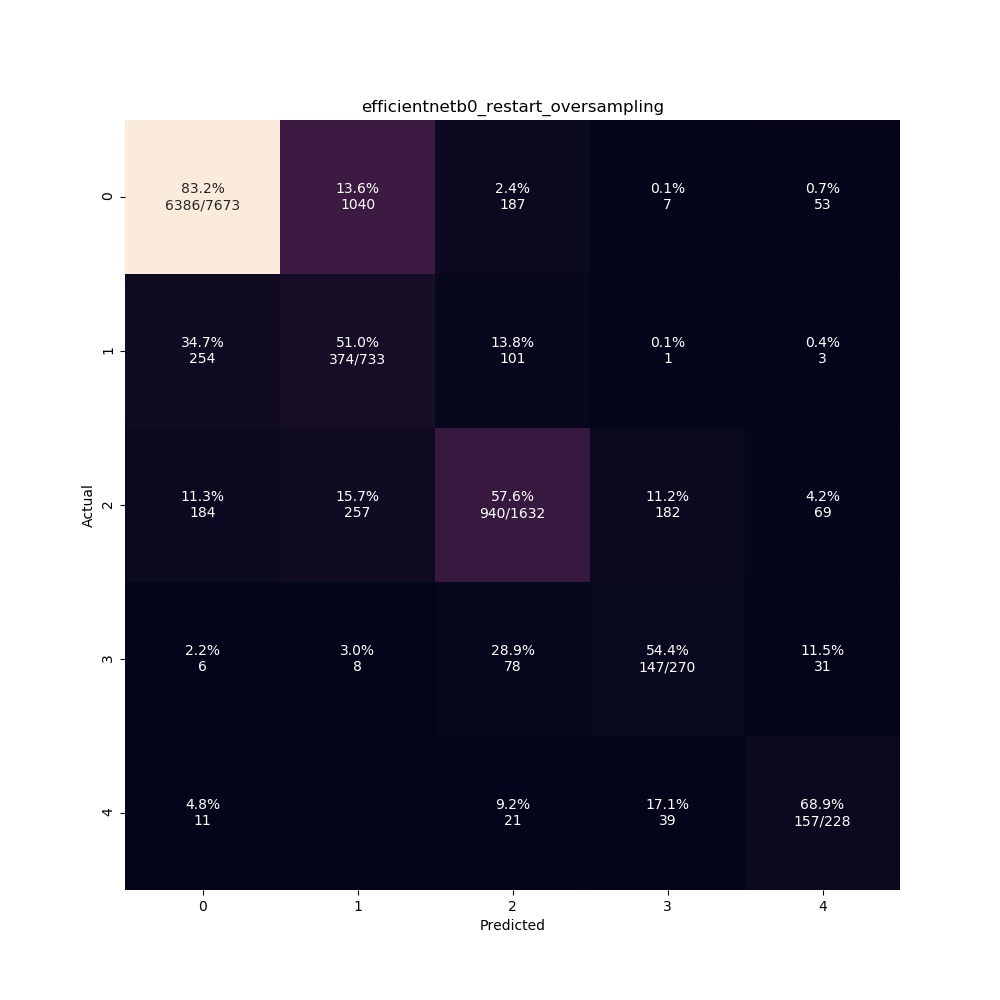
\includegraphics[width=1\linewidth]{efficientnetb0_restart_oversampling.jpeg}
\subcaption{}
\end{minipage}
\begin{minipage}{5cm}
\centering
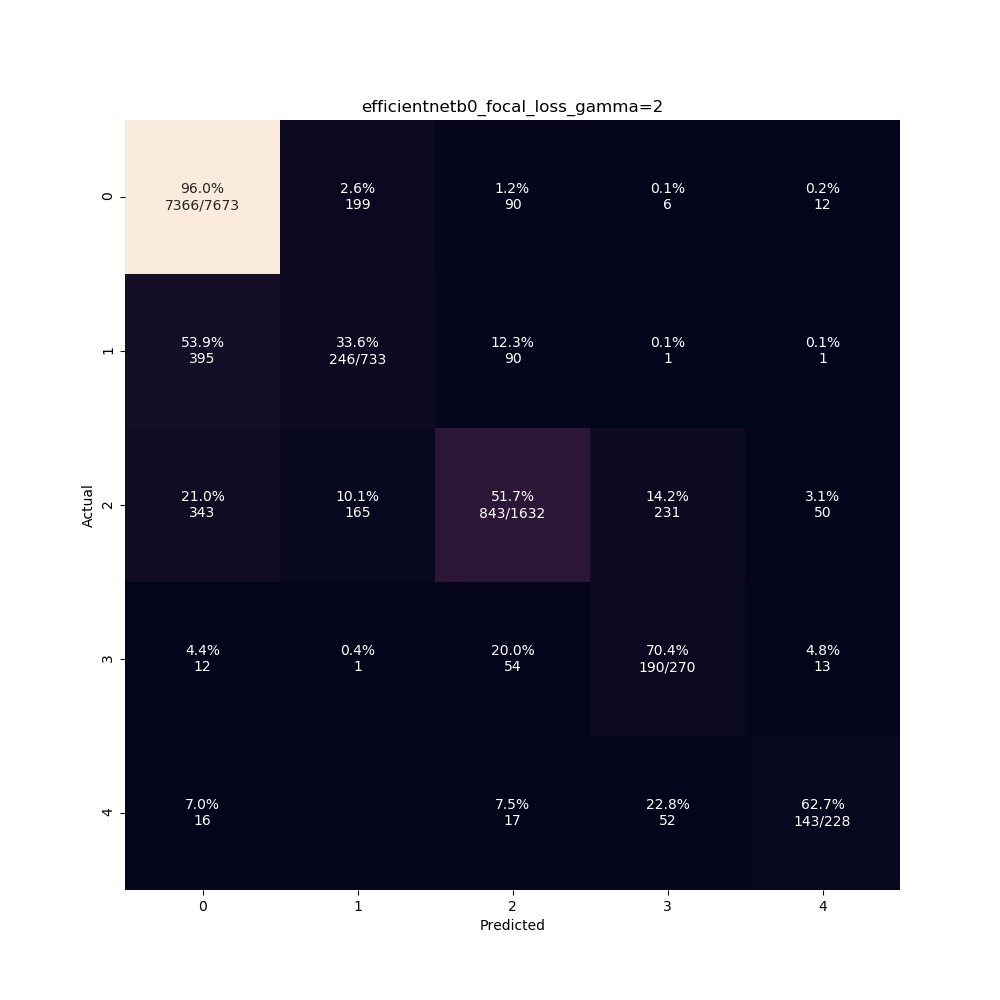
\includegraphics[width=1\linewidth]{efficientnetb0_focal_loss.jpeg}
\subcaption{}
\end{minipage}
\begin{minipage}{5cm}
\centering
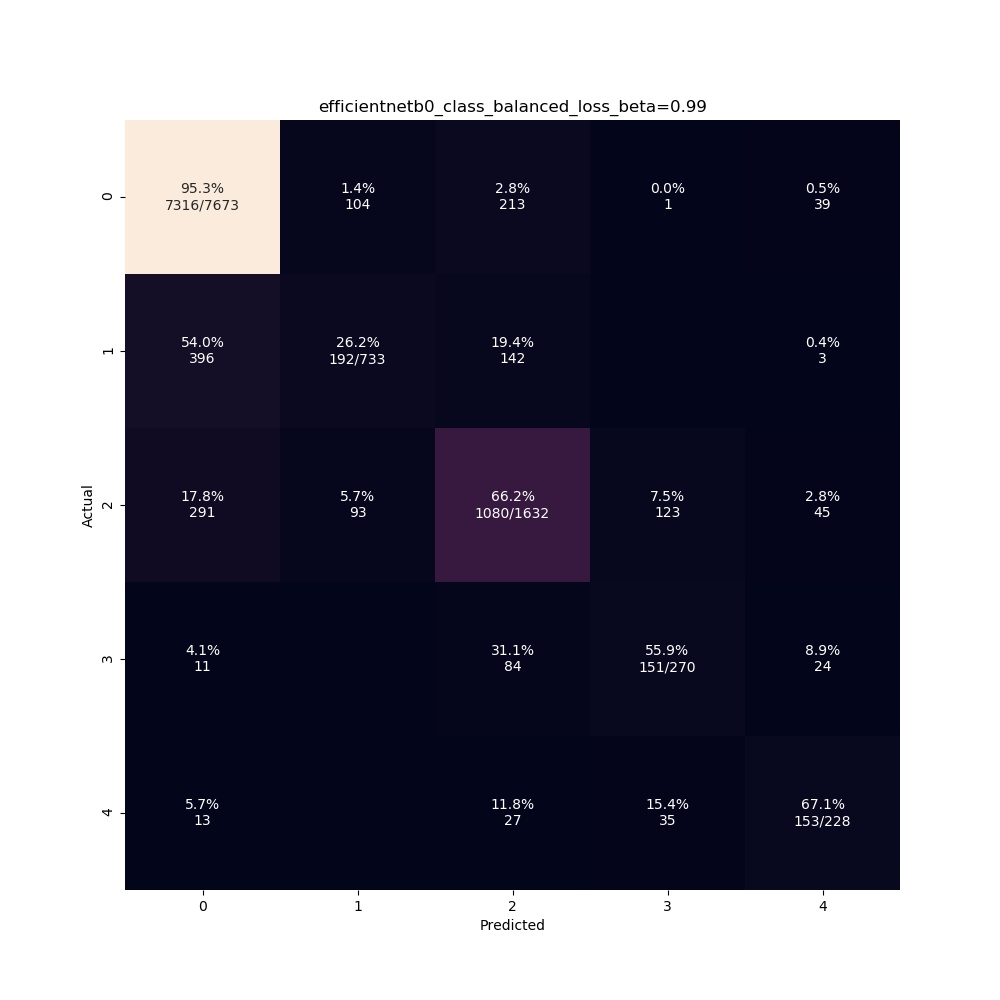
\includegraphics[width=1\linewidth]{efficientnetb0_class_balanced_loss.jpeg}
\subcaption{}
\end{minipage}
\caption{Comparison of confusion matrices of efficient b0 trained on imbalanced dataset(a), on oversampled balanced dataset with dropout rate=0.9(b), on oversampled balanced dataset starting from pre-trained weights(c), on imbalanced dataset using focal loss with $\gamma$=2(d) and on imbalanced dataset with $\beta$=0.99(e). The matrices are obtained by testing on the 30\% validation dataset.}
\label{fig:confusion_imbalanced}
\end{figure}
\newpage
%------------------------------------------Corrupted Images--------------------------------------------------------------------
\section{Training with Corrupted Images}
In view of equipping the model with robustness against low-quality or even corrupted images, we train the model on a dataset of images that undergo different types of corruptions(light leakage, motion blur, under expose and over expose) at different levels (from 1 to 4, the higher the level, the worse the images). The effects of corruptions are demonstrated in figure\ref{fig:corruptions}. The corruption processing is Zeiss-proprietary. 

The training is proceeded using the same training-validation split as the above sections. The baseline model is efficientnet b0, the images are of size 512$\times$512, the batch size is set to be 48 and dropout is not used.

Although the underlying corruptions can be served as a new data augmentation and be applied newly to each image at each epoch, due to the lengthy image processing which takes around 50 seconds per image, we process the images of the (oversampled) original dataset and save them as new datasets. No other data augmentation is added. The corrupted datasets are then directly loaded for training without any further operation. During the generation of the corrupted datasets, four types of corruptions are randomly applied with random parameters that conform to their randomly chosen level in the level range. 

\textbf{Test on original validation set}. The results on the original imbalanced dataset and oversampled balanced dataset obtained after 20 epochs and validated on the untouched imbalanced validation set are respectively summarised in table\ref{tab:corruptions_imbalanced} and table\ref{tab:corruptions_balanced}. Compared with model trained on imbalanced dataset, we notice a drop in performance of the model because of the loss of information due to corruption. Nonetheless, when acting on an oversampled balanced dataset, the corruptions play a role of an enhanced data augmentation that mitigates the problem of overfitting. 

\textbf{Test on corrupted validation set}. To check if training on a corrupted dataset can bestow resistance to corruption on the model, we further test the models on corrupted imbalanced validation dataset whose corruption level range is 1 -- 4. The results are listed in table\ref{tab:valid_corrupted}. 

As revealed in the results, training on a corrupted dataset allows the model to gain robustness against the corruptions of the same types. 

\textbf{Resistance against adversarial attack}. To investigate the ability of the corrupted-trained model to withstand an adversarial attack, we measure such ability by recording the success rate of an attack at different “box size" $\epsilon$ of the $l_{\infty}$ PGD attack\cite{madry_towards_2017}. The success rate of an attack is defined by the number of the change of predictions after the attack over the total number of samples. Briefly speaking, $\epsilon$ represents the size of the box in the sample space inside which the adversarial samples are searched. As a result, the greater $\epsilon$ is, the larger the box will be, the stronger the attack will be and the higher the success rate will be. At the same $\epsilon$, if the success rate of an attack is higher, the model is considered to be weaker against the attack.

The experiment is performed on 240 samples randomly chosen from the original validation set, the number of steps of the PGD attack is set to be 5 .

Results are presented in table\ref{tab:corrupted_adv}. It turns out that training on corrupted dataset does not seem to help the model gain resistance against gradient-based adversarial attacks. On the contrary,  the corrupted-trained model becomes more vulnerable in face of such attacks. This behaviour might be due to the fact that corrupted images still contain some non-robust features while lose some robust features of the original images. Consequently,  compared with baseline, the model learns some non-robust features of the corrupted images and at the same time have no access to certain robust features of the original dataset, which results in a worse performance on adversarial samples generated from the original dataset. It would be better if the model is trained on a mixed dataset where both original and corrupted images are present.

\begin{figure}[htbp]
\captionsetup{margin=5mm,justification=justified,font=small,labelfont=bf,textfont = it, margin={10mm,0mm}}
\centering
\begin{minipage}{5cm}
\centering
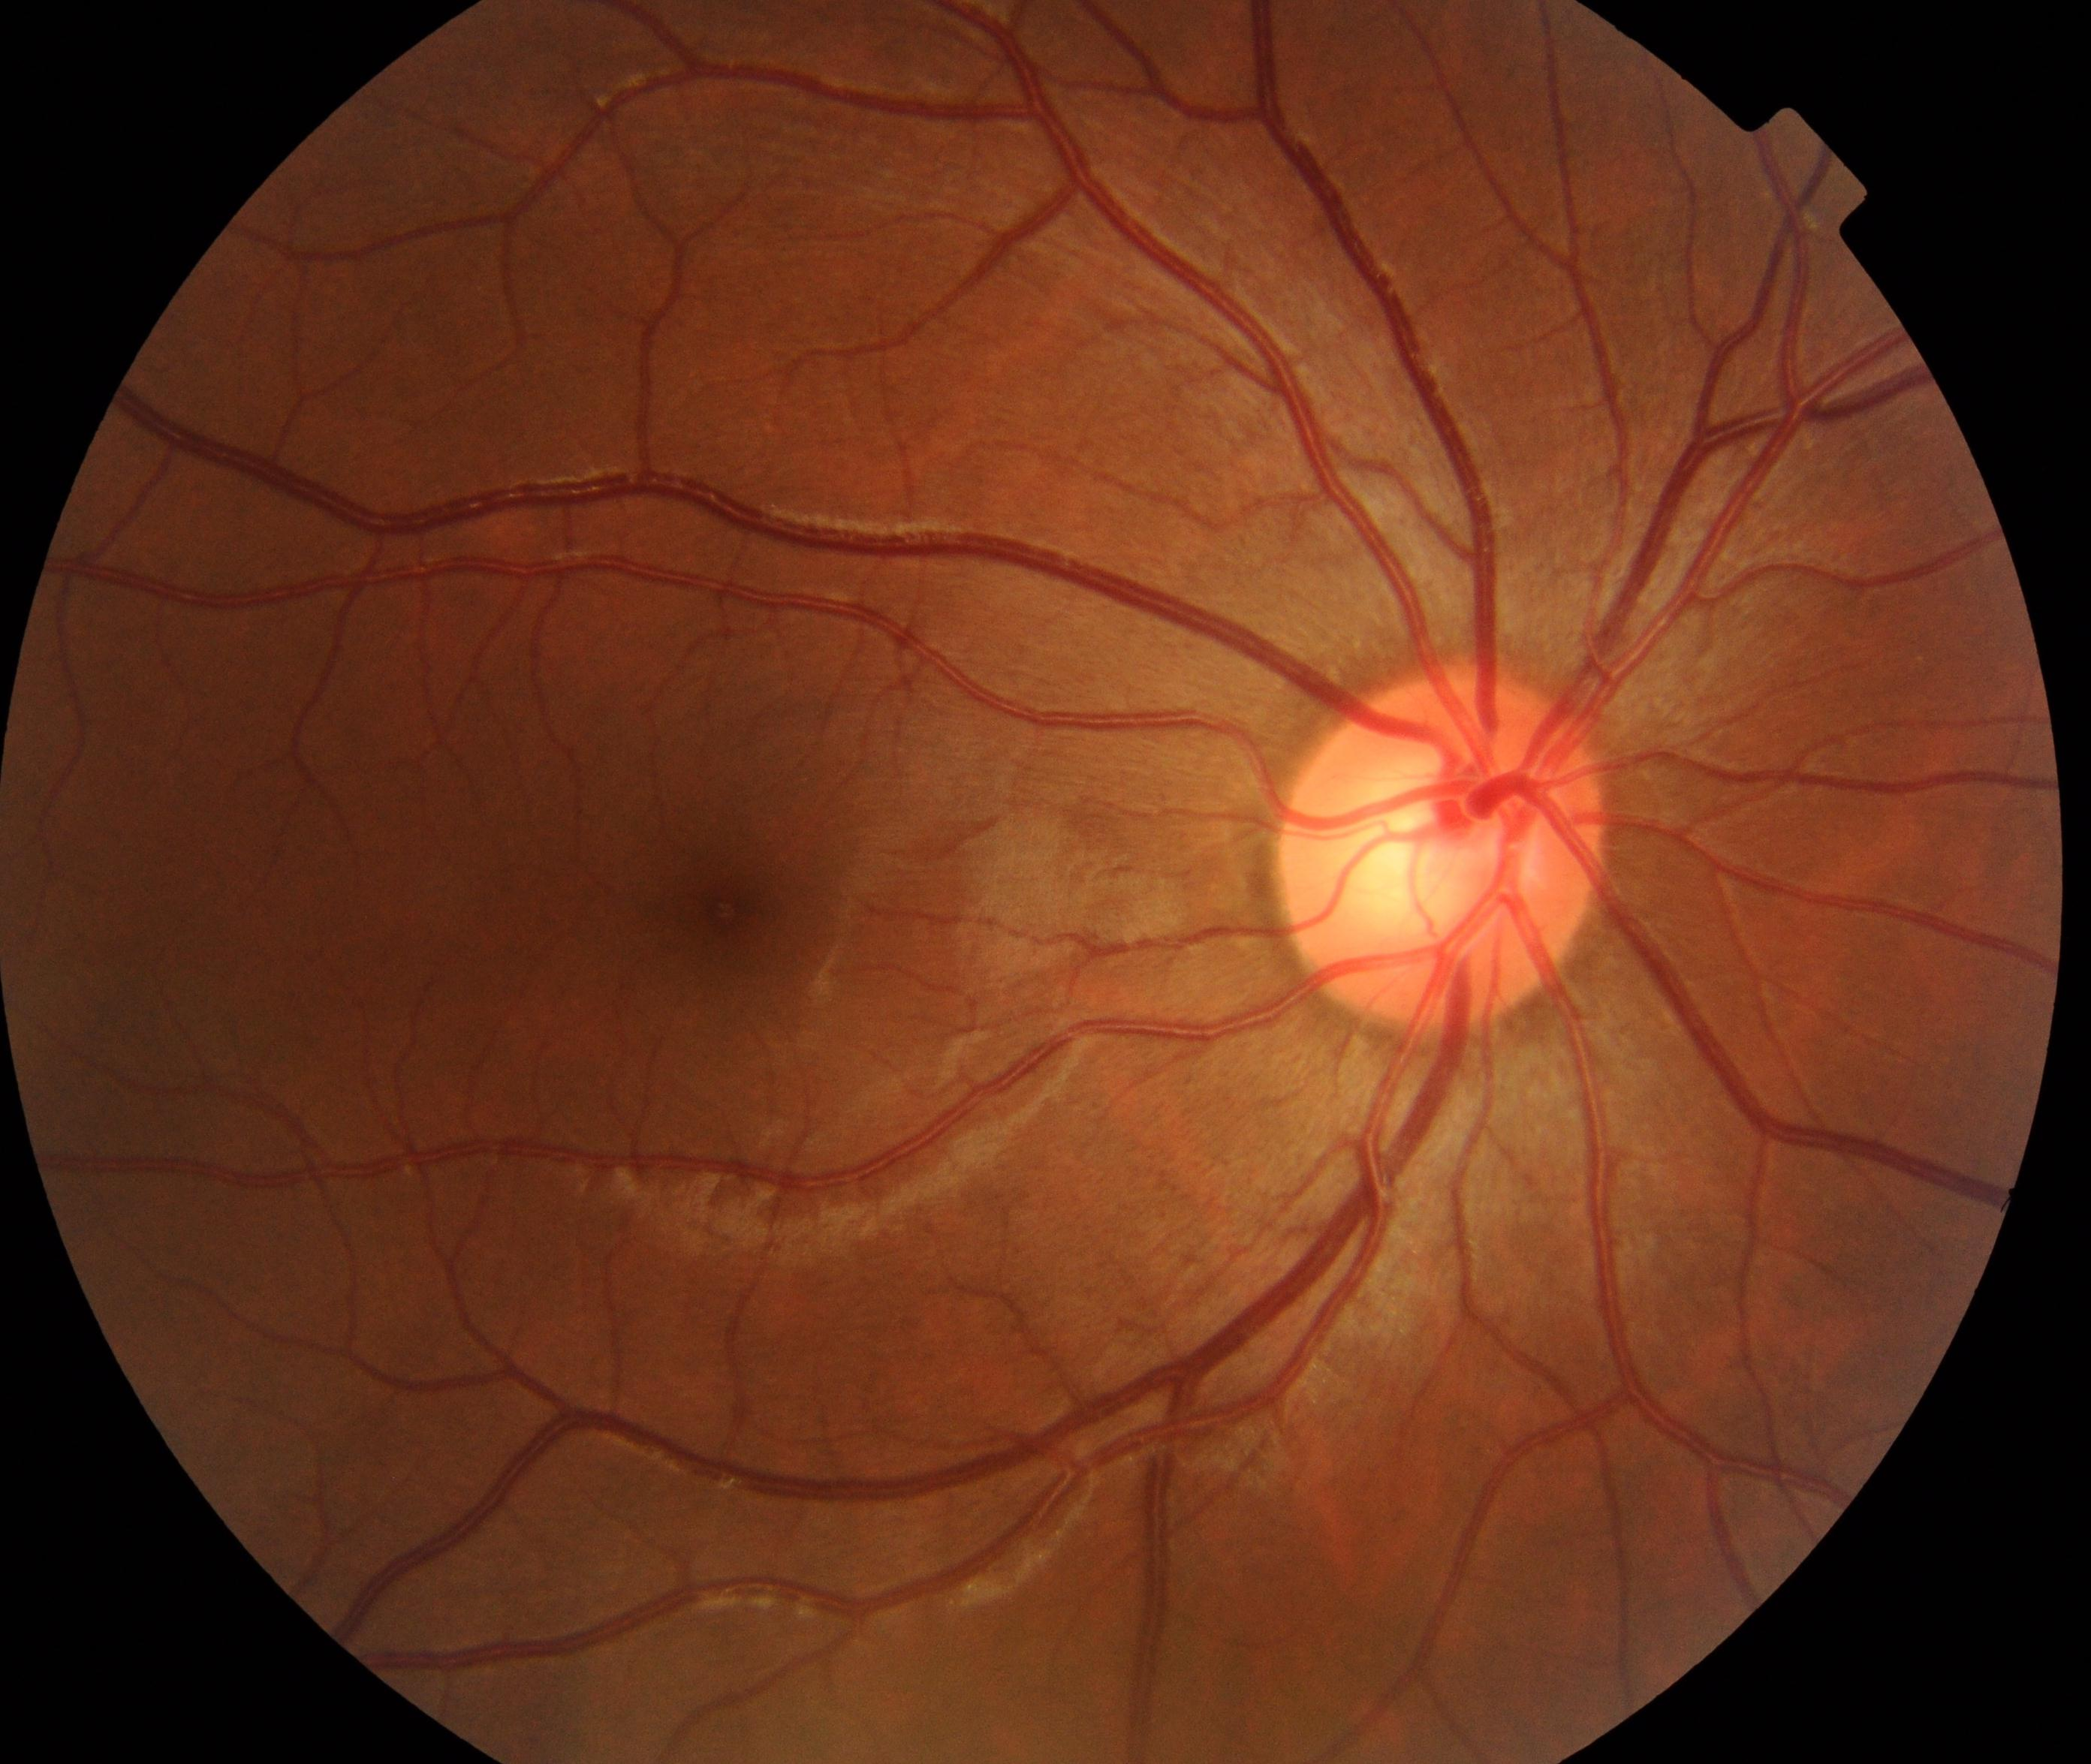
\includegraphics[width=1\linewidth]{testimage.jpg}
\subcaption{}
\end{minipage}
\begin{minipage}{5cm}
\centering
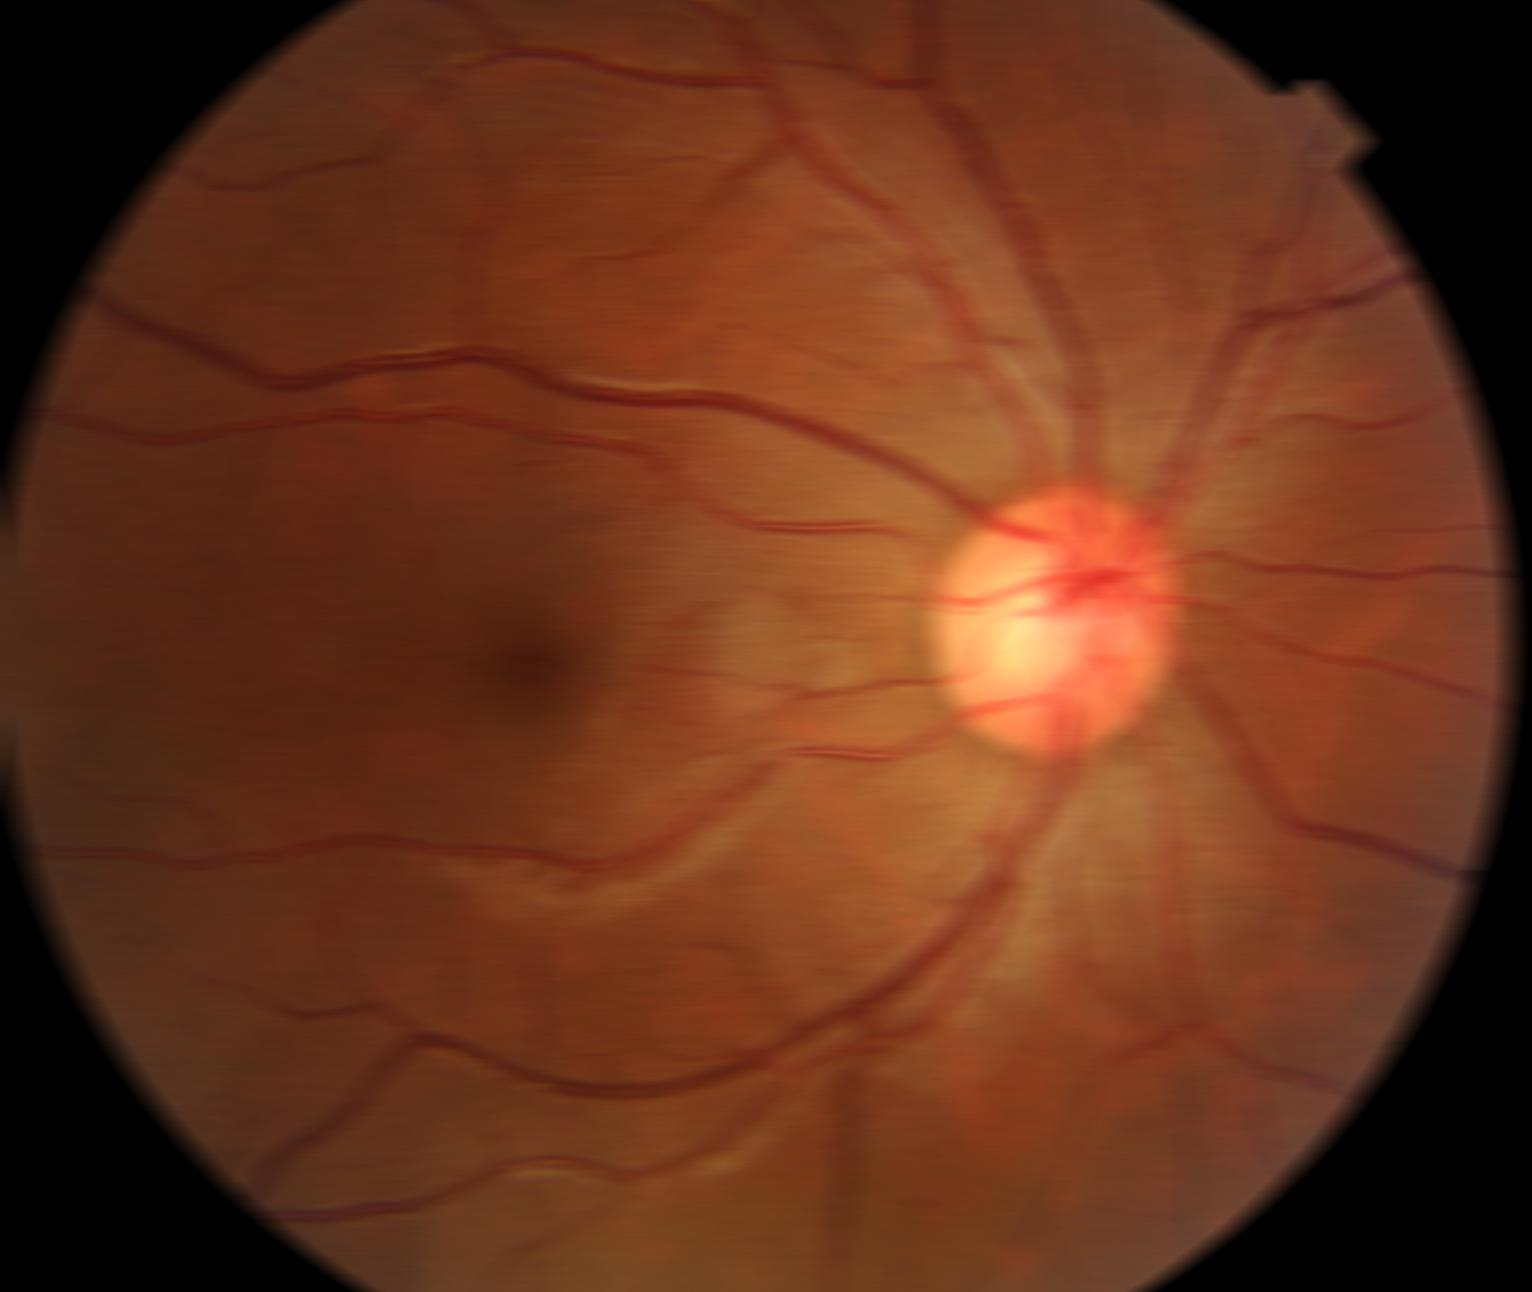
\includegraphics[width=1\linewidth]{testimage_augmented__1.jpg}
\subcaption{}
\end{minipage}
\begin{minipage}{5cm}
\centering
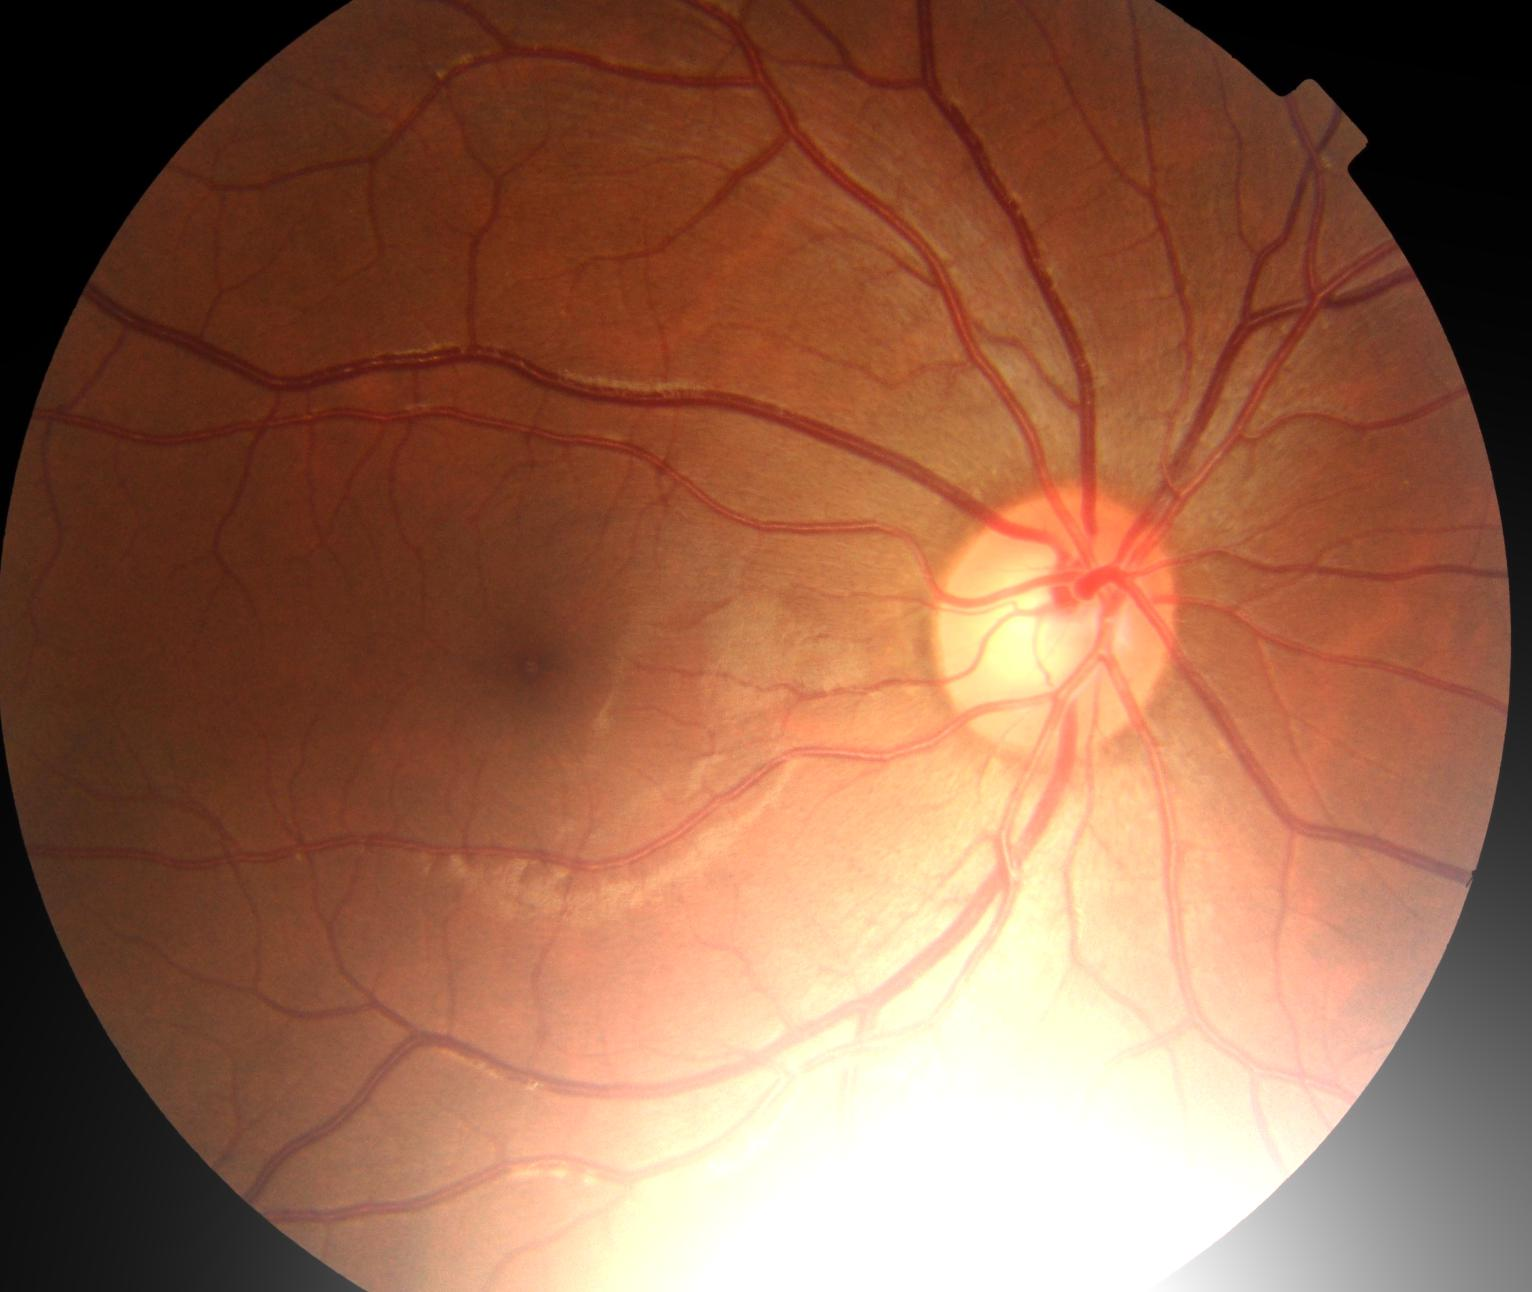
\includegraphics[width=1\linewidth]{testimage_augmented__10.jpg}
\subcaption{}
\end{minipage}
\begin{minipage}{5cm}
\centering
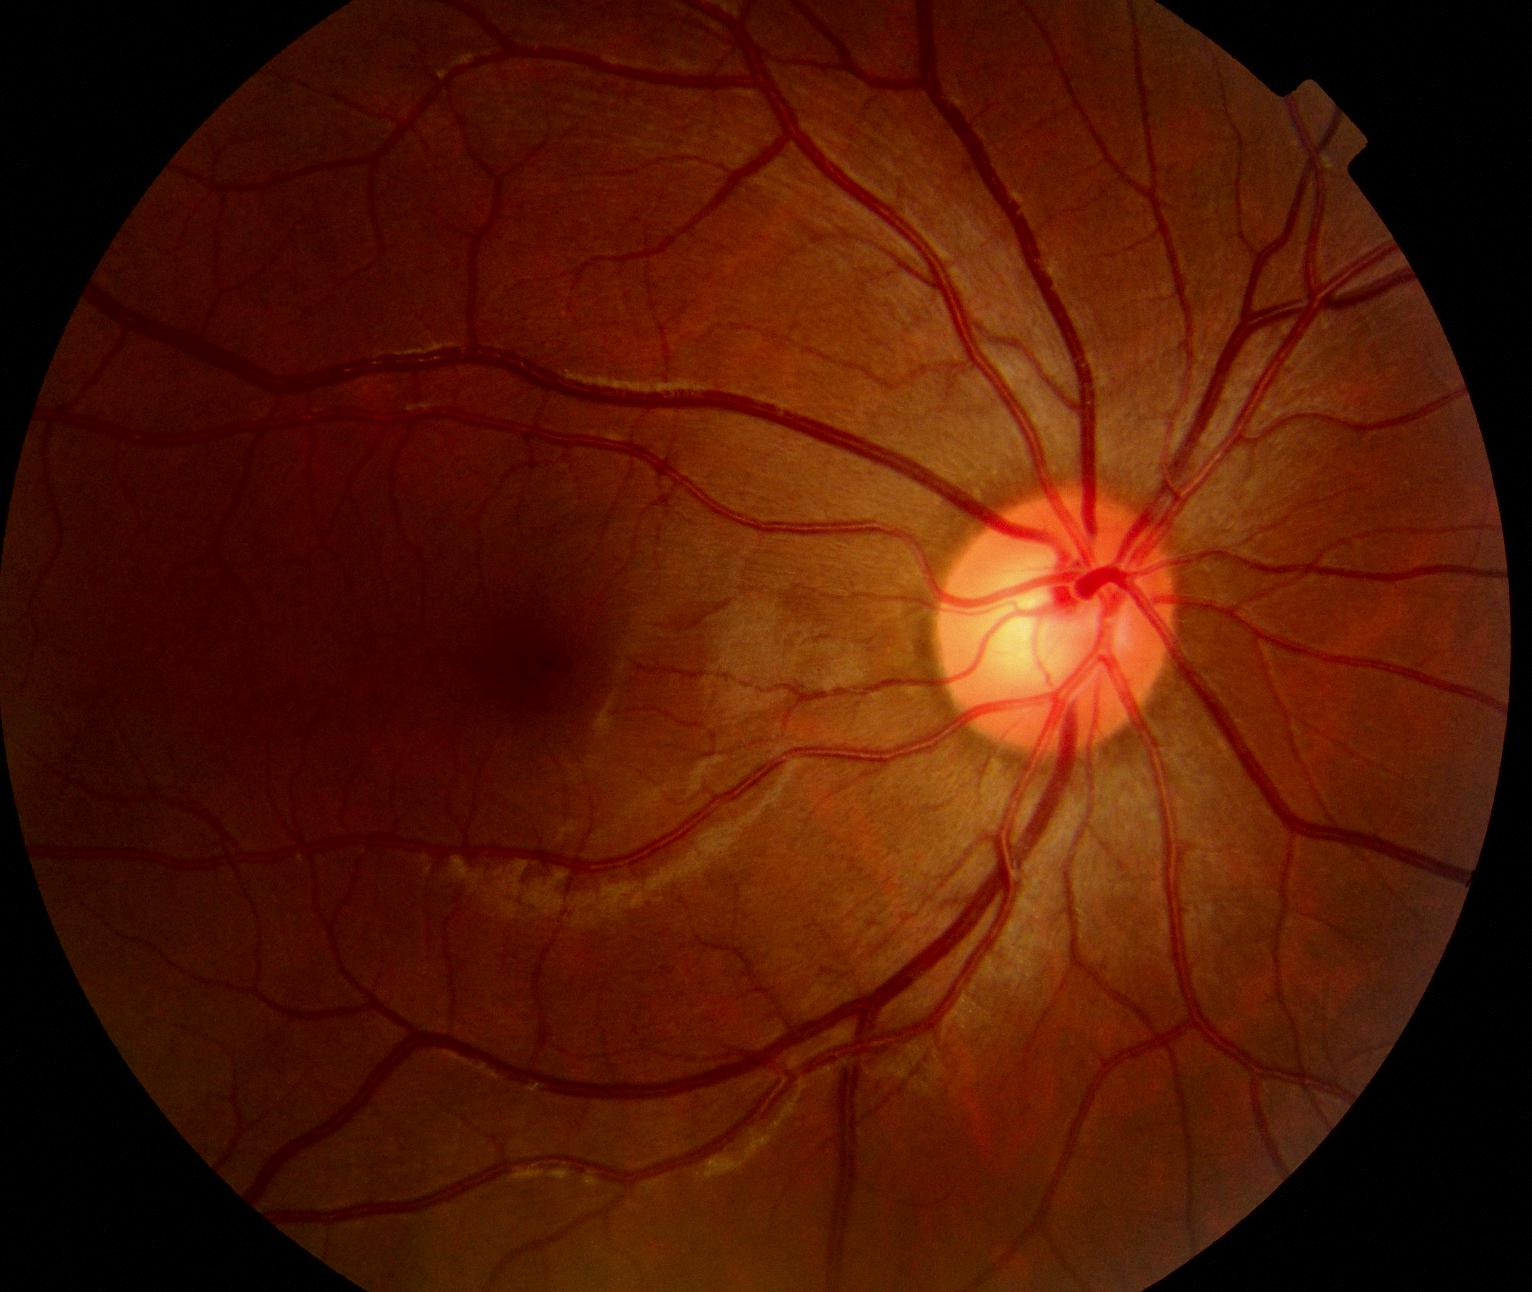
\includegraphics[width=1\linewidth]{testimage_augmented__9.jpg}
\subcaption{}
\end{minipage}
\begin{minipage}{5cm}
\centering
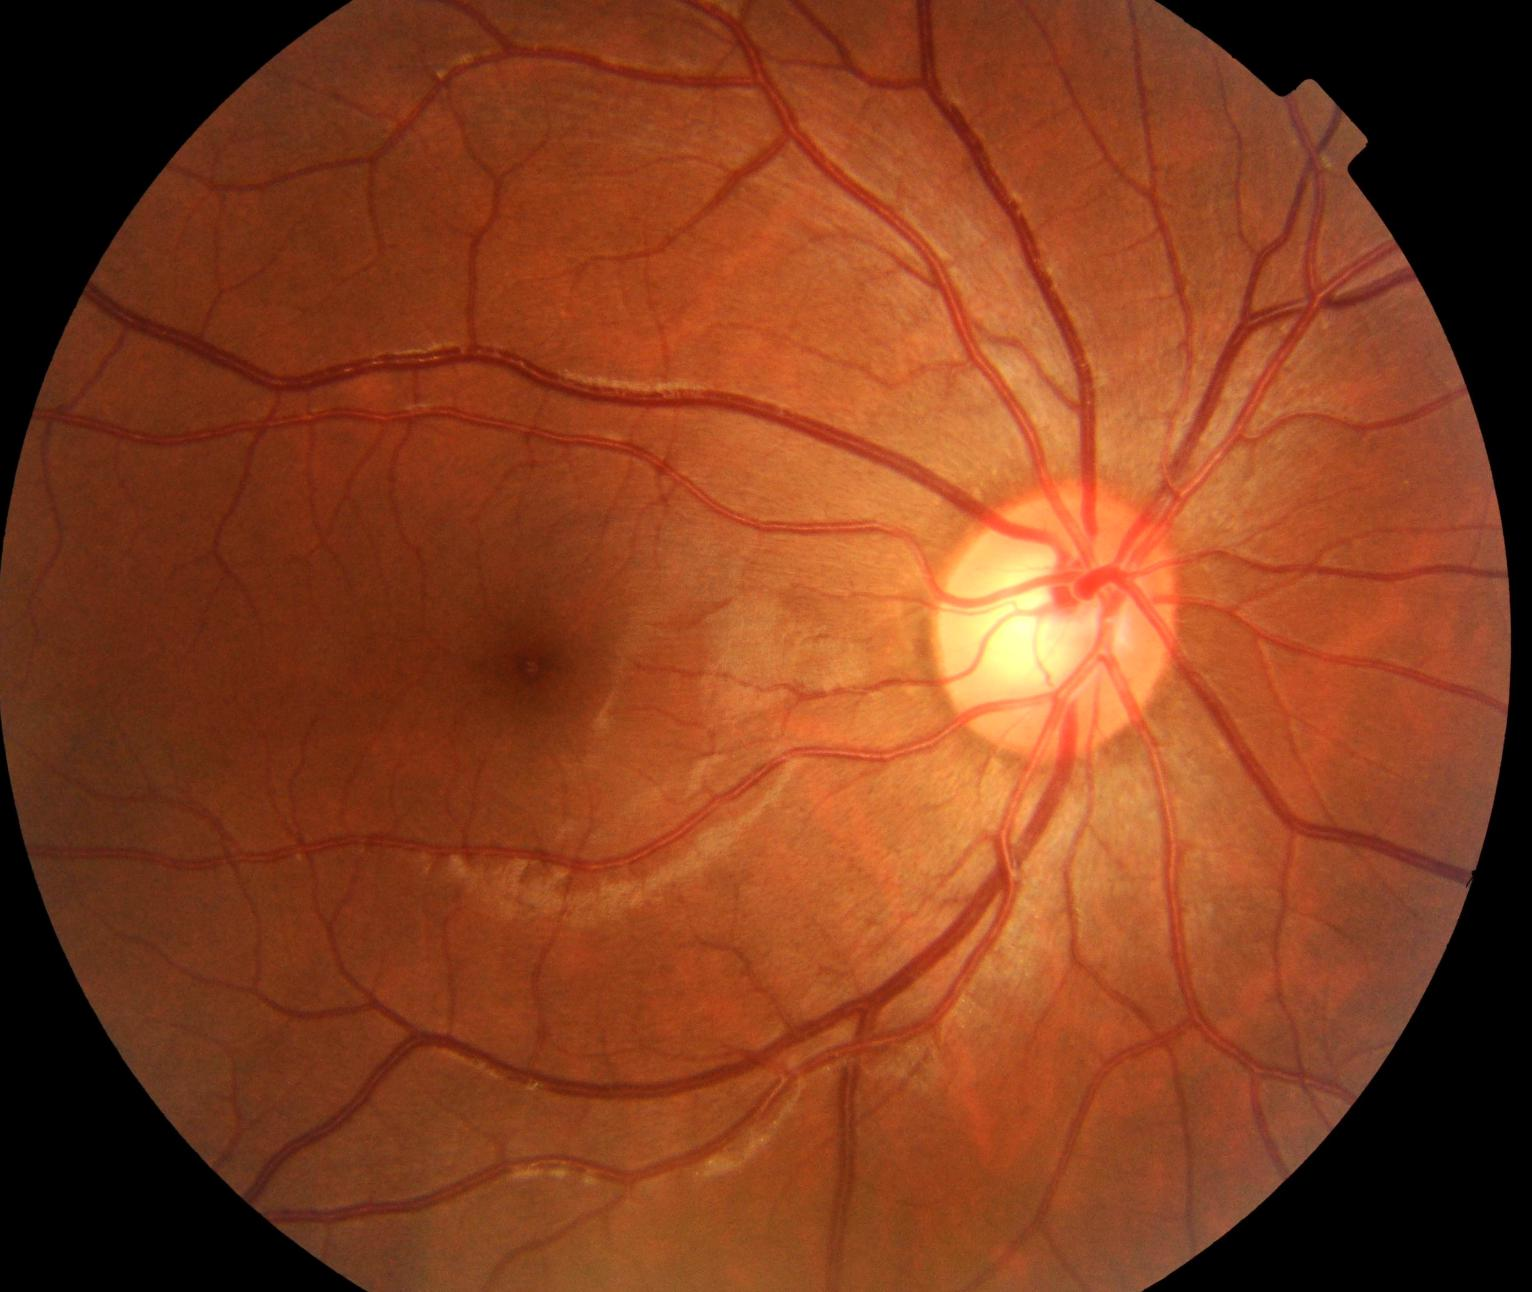
\includegraphics[width=1\linewidth]{testimage_augmented__14.jpg}
\subcaption{}
\end{minipage}
\caption{Different kinds of corruptions on a test image(a): motion blur(b), light leakage(c), under expose(d) and over expose(e).}
\label{fig:corruptions}
\end{figure}

\begin{table}[htbp]
\linespread{1.5} 
\renewcommand\arraystretch{1.25}
\captionsetup{margin=5mm,justification=justified,font=small,labelfont=bf,textfont = it, margin={10mm,0mm}}
\centering
\begin{tabular}{|c|c|c|c|}
    \hline
     Corruption Level Range& Accuracy & Balanced Accuracy & Cohen Kappa Score\\
     \hline
     baseline & 0.852 & 0.586. & 0.805 \\
     \hline
     1 & 0.812 & 0.475 & 0.701   \\
     \hline
     1 -- 2& 0.817 & 0.497 & 0.725\\
     \hline
     1 -- 3& 0.826 & 0.500 & 0.718  \\
     \hline
     1 -- 4& 0.817 & 0.515 & 0.731 \\
     \hline
\end{tabular}
\caption{Performance of efficient b0 trained on imbalanced dataset at different level ranges}
\label{tab:corruptions_imbalanced}
\end{table}


\begin{table}[htbp]
\linespread{1.5} 
\renewcommand\arraystretch{1.25}
\captionsetup{margin=5mm,justification=justified,font=small,labelfont=bf,textfont = it, margin={10mm,0mm}}
\centering
\begin{tabular}{|c|c|c|c|}
    \hline
     Training Corruption Level Range& Accuracy & Balanced Accuracy & Cohen Kappa Score\\
     \hline
     baseline & 0.704 & 0.399 & 0.612 \\
     \hline
     1 & 0.806 & 0.477 & 0.705   \\
     \hline
     1 -- 2& 0.812 & 0.471 & 0.703\\
     \hline
     1 -- 3& 0.807 & 0.481 & 0.707  \\
     \hline
     1 -- 4& 0.803 & 0.466 & 0.695 \\
     \hline
\end{tabular}
\caption{Performance of efficient b0 trained on balanced dataset at different level ranges}
\label{tab:corruptions_balanced}
\end{table}

\begin{table}[htbp]
\linespread{1.5} 
\renewcommand\arraystretch{1.25}
\captionsetup{margin=5mm,justification=justified,font=small,labelfont=bf,textfont = it, margin={10mm,0mm}}
\centering
\begin{tabular}{|c|c|c|c|c|}
    \hline
     Training Corruption Level Range& Accuracy & Balanced Accuracy & Cohen Kappa Score & Accuracy Drop\\
     \hline
     baseline & 0.764 & 0.391 & 0.501& 0.088 \\
     \hline
     1 & 0.778 & 0.417 & 0.575  & 0.034 \\
     \hline
     1 -- 2& 0.785 & 0.446 & 0.619 & 0.032\\
     \hline
     1 -- 3& 0.776 & 0.393 & 0.586  & 0.050\\
     \hline
     1 -- 4& 0.791 & 0.403 & 0.598 & 0.026\\
     \hline
\end{tabular}
\caption{Performance of corrupted-trained efficient b0s on corrupted(1 -- 4) imbalanced validation dataset}
\label{tab:valid_corrupted}
\end{table}

\begin{table}[htbp]
\linespread{1.5} 
\renewcommand\arraystretch{1.25}
\captionsetup{margin=5mm,justification=justified,font=small,labelfont=bf,textfont = it, margin={10mm,0mm}}
\centering
\begin{tabular}{|c|c|c|c|}
    \hline
     Training Corruption Level Range& $\epsilon$=0.2 & $\epsilon$=0.4 & $\epsilon$=0.6  \\
     \hline
     baseline & 0.196& 0.238& 0.341 \\
     \hline
     1 & 0.467& 0.867 &  0.896\\
     \hline
     1 -- 2& 0.588 & 0.875& 0.883  \\
     \hline
     1 -- 3& 0.554 & 0.867 & 0.871   \\
     \hline
     1 -- 4& 0.579 & 0.871& 0.879  \\
     \hline
\end{tabular}
\caption{Success rate of PGD attack at different $\epsilon$ for different models }
\label{tab:corrupted_adv}
\end{table}


\end{document}
